%!TEX root = /Users/laura/Repositories/HandwritingRecognition/report/main.tex
	\begin{figure}[t]
		\centering
		\subfloat[]{
			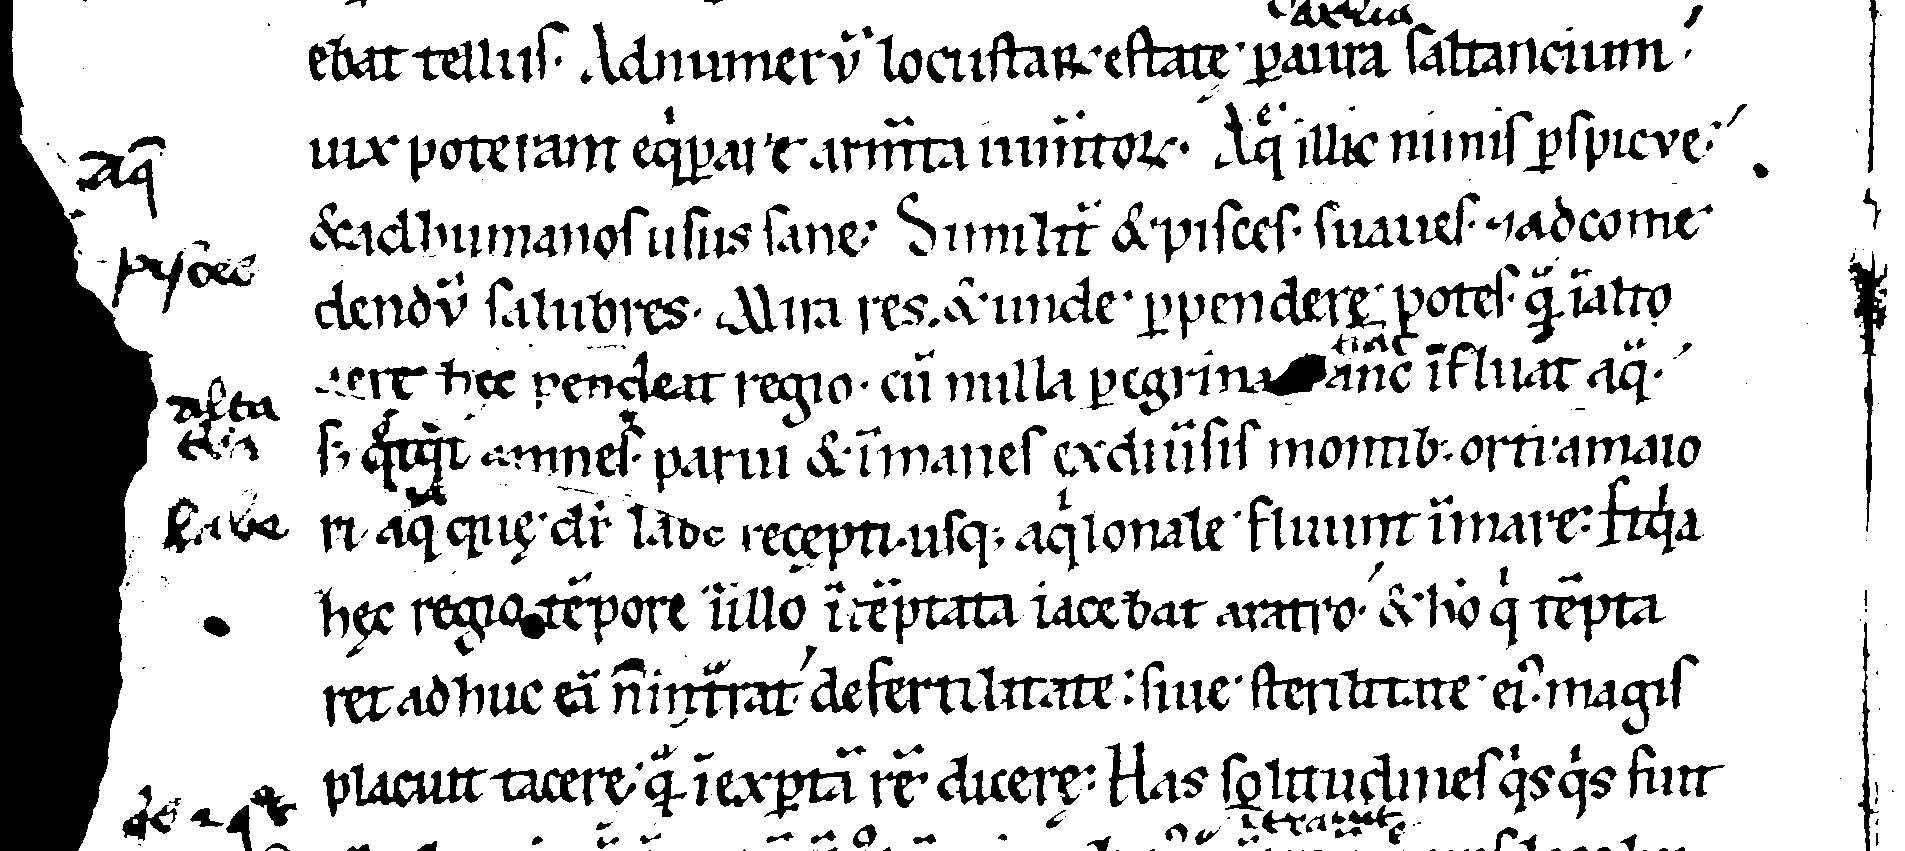
\includegraphics[width=0.6\columnwidth, height=0.1\textheight, keepaspectratio]{individual/img/discussion/bohemians.png}%
			\label{fig:discussion:preprocessing:bohemians}%
		}
		\hfil
		\subfloat[]{
			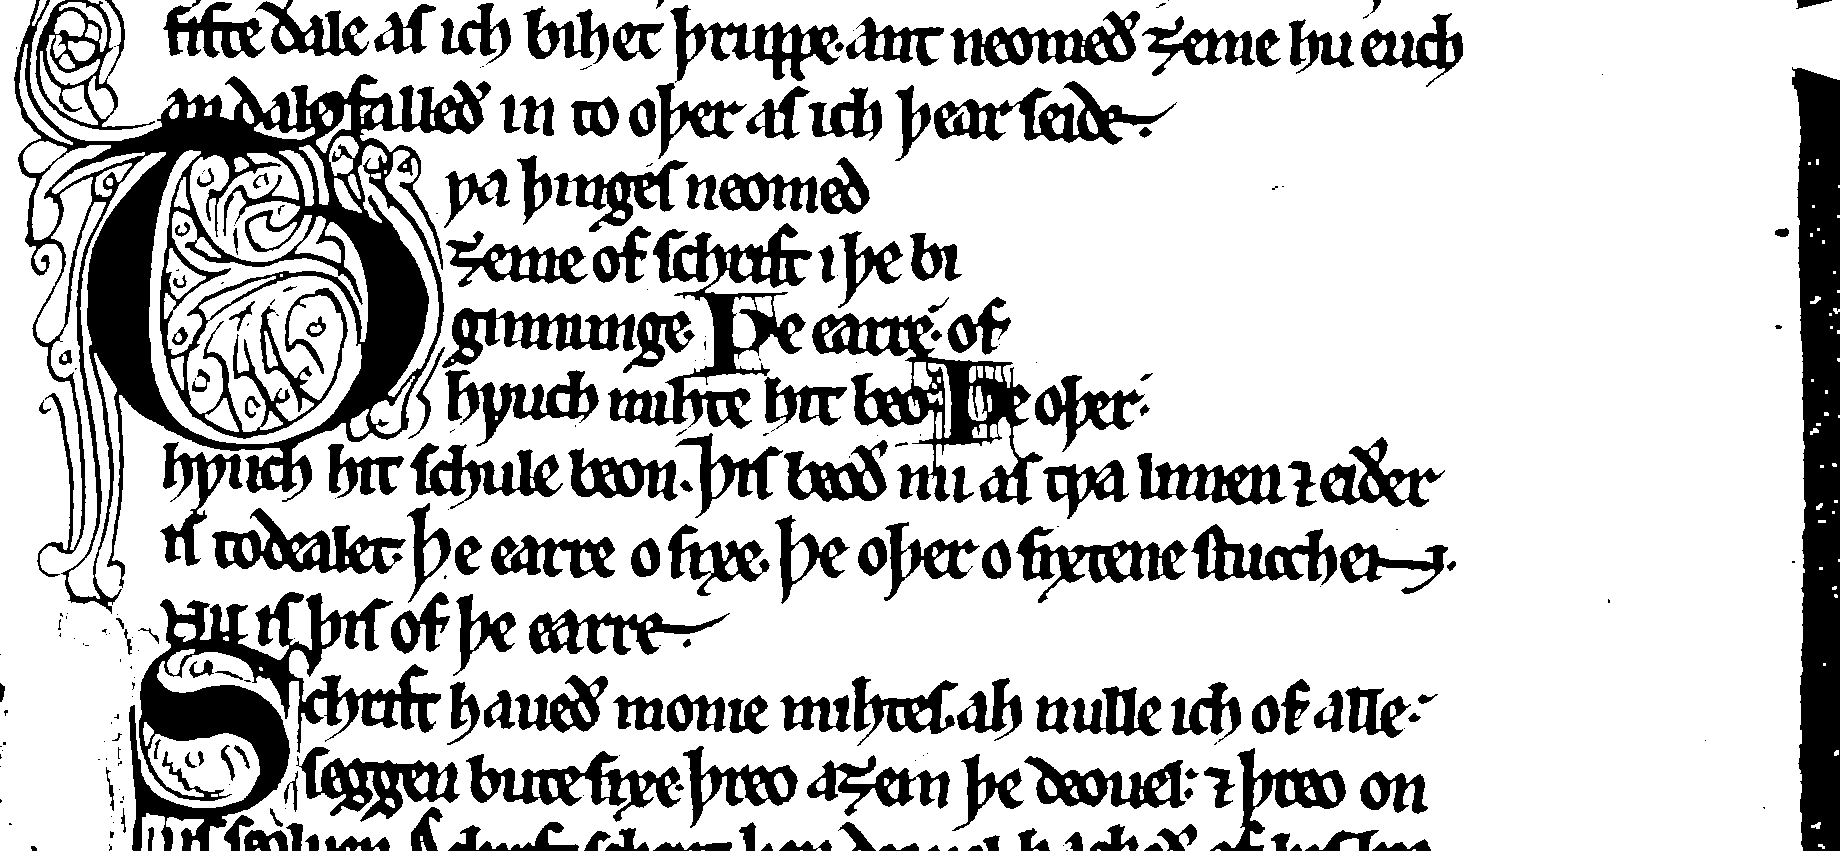
\includegraphics[width=0.6\columnwidth, height=0.1\textheight, keepaspectratio]{individual/img/discussion/oldEnglishHomilies.png}%
			\label{fig:discussion:preprocessing:oldEnglishHomilies}%
		}
		\caption{Part of a preprocessed page from \protect\subref{fig:discussion:preprocessing:bohemians} ``Chronicle of the Bohemians" and \protect\subref{fig:discussion:preprocessing:oldEnglishHomilies} ``Old English Homilies".}
		\label{fig:discussion:preprocessing:preprocessedExampleData}
	\end{figure}
\Cref{fig:discussion:preprocessing:preprocessedExampleData} shows the preprocessed versions of the images shown in \cref{fig:introduction:exampleData}. Comparing \cref{fig:introduction:bohemians} with \ref{fig:discussion:preprocessing:oldEnglishHomilies} the letter boundaries in the second are much clearer than the boundaries in the first. This could explain why the error on ``Chronicle of the Bohemians" is lower than on the other data set. 